\cotefile{84}
\scanpage{97}

\diagram{\begin{tikzcd}[ampersand replacement=\&,column sep=large]
0\arrow[r] \& L\arrow[r,dash]\arrow[d,"{-\mathrm{id}}"] \& E\arrow[r]\arrow[d,"g","?"'] \& \underline{\mathcal O}\arrow[r]\arrow[d,"\mathrm{id}"] \& 0\\
0\arrow[r,dash] \& L\arrow[r] \& A\otimes L\arrow[r,"{\varphi\otimes\mathrm{id}_{L}}"] \& \underline{\mathcal O}\arrow[r] \& 0
\end{tikzcd}}

\margin{Attention au signe $\longrightarrow$}

Prouvons d'abord

\[
\varphi\otimes\mathrm{id}_{L}\bigl(\underbrace{g(x)}_{\substack{\rotatebox{90}{$\in$}\\ \deleted{\unsure{\mathrm{H}|\mathrm{Hom}}}A\otimes L=\mathrm{Hom}(E,L)}}\bigr)=\psi(x)
\qquad \forall x\in\Gamma(E)
\]

Cela signifie que $\forall x\in E$,

\[
g(x)|L=(u\longmapsto\psi(x)u)
\]

\deleted{\illegible{1}} i.e. on a

\[
\underset{\substack{\Vert\\ \psi(x).u-\underset{\substack{\Vert\\0}}{\psi(u)}x}}{g(x)(u)}
=\psi(x)u\qquad\text{pour tout }u\in\Gamma L\subset\Gamma E
\]

c'est OK.

Prouvons ensuite que pour $x\deleted{\unsure{\in E}}\in\Gamma L$, on a $g(x)\unsure{:}E\longrightarrow L$ est \uline{nul} sur $L$, et par passage au quo. induit $\lambda\longmapsto-\lambda x$ de $\mathcal O$ en \unsure{$x$|$L$},

\margin{signe $\nearrow$}

\[
\text{i.e.}\qquad g(x)(y)=-\psi(y)x,
\]

mais c'est aussi OK.

Ceci vu, l'isom. d'ext. $g$ définit

\[
\mathrm{Quad}(E,L^{\otimes2})\simeq\mathrm{Quad}(A,\mathcal O)
\]

\deleted{$\unsure{\mathrm{Sym}^{\! \unsure{2|4}}|\mathrm{Quad}}( \check E)\otimes L^{\otimes2}\qquad \unsure{\mathrm{Sym}^{2}}$}.

% slanted
\uline{dis que \inserted{lorsque $E$ provient d'un \unsure{rev.} du \unsure{1\textsuperscript{er}} type, d'où $N$ sur $A$, $Q$ sur $E$, alors} par cet} iso, \uline{$N$ et} \uline{$Q$ se} \uline{correspondent}. Pour le prouver, OPS $E$ scindé en

\[
E\simeq L\oplus\underline{\mathcal O}.x_0
\]

\[
\text{d'où}\qquad A\simeq\underline{\mathcal O}\oplus L^\vee \qquad
\text{i.e.}\quad A\otimes L\simeq L\oplus
\underbrace{L\otimes L^\vee}_{\underline{\mathcal O}_X}
\]

% archive sheet number: 96

\scanpage{98}

et l'isom $E\longrightarrow\deleted{\unsure{E}}A\otimes L$ respecte les décompositions en somme directe

\diagram{\begin{tikzcd}[ampersand replacement=\&,column sep=small]
\deleted{\unsure{A}}E={} \& \underline L\arrow[d,"{-\mathrm{id}_{L}}"] \& {}\oplus{} \& \underline{\mathcal O}.x_0\arrow[d,dash,"\mathrm{id}"]\\
A\otimes L\simeq{} \& \underline L \& {}\oplus{} \& \underline{\mathcal O}.
\end{tikzcd}}

Si donc $Q$ est donnée par

\[
Q(\underset{\substack{\rotatebox{90}{$\in$}\\\Gamma L}}{u}+\lambda x_0)
=u^2+\lambda\deleted{\unsure{x}}\langle u,\underset{\substack{\rotatebox{90}{$\in$}\\\Gamma L}}{b}\rangle
+\lambda^2\underset{\substack{\rotatebox{90}{$\in$}\\\Gamma L^{\otimes2}}}{c},
\]

le signe $-\mathrm{id}_{L}$ sur le diagramme précédent implique que l'on aura

\[
N(\underset{\substack{\rotatebox{90}{$\in$}\\\Gamma L^\vee}}{v}+\deleted{\unsure{=}}\lambda 1)
=\deleted{\unsure{v^2}}\lambda^2\deleted{\unsure{+}}-\lambda\langle v,b\rangle+\langle v^{2},c\rangle
\]

La formule

\[
\boxed{Q_N(\varphi_N(x))=-N(x)\delta_N}
\]

(les deux mbres sont des \unsure{3|S}-formes p.r. à l'argument $N$ variable\ldots) est bien sûr valable dans le contexte général d'un mod. loc. libre $A$ \inserted{de rang $2$} et d'une forme quadratique \deleted{\unsure{invol.}} $N$ dessus, sans \unsure{autre donnée|autres données}.

\figure{\begin{tikzpicture}\draw (0,0)--(.35,-.95);\end{tikzpicture}}

% archive sheet number: 97

\scanpage{99}

Comme $A_i\simeq E_i\otimes L_i^\vee$, $A\simeq{}E\otimes L^\vee$, on \unsure{a donc|aura|trouve}

\[
E\otimes L^\vee\longleftrightarrow(E_1\otimes L_1^\vee)\unsure{\ominus|\otimes}(E_2\otimes L_2^\vee)
\]

et comme

\[
L^\vee\simeq L_1^\vee\otimes L_2^\vee,
\]

on en déduit également

\[
E\xrightarrow{i}E_1\otimes E_2
\]

qui est une sorte de \unsure{transposé|transposée} de $E_1\otimes E_2\longrightarrow E$.

\margin{$x_1\otimes x_2\longmapsto x_1*x_2$\,\unsure{;|:}}

\deleted{Pour \deleted{\unsure{ex}}expliciter $i$, il faut donner les deux composés $\overset{\alpha=}{i\circ *},\ \overset{\beta=}{i\circ\mathrm{inj}}$,}

\diagram{\begin{tikzcd}[ampersand replacement=\&,column sep=small]
\deleted{E_1\otimes E_2}\arrow[dr,"*"']\arrow[rrd,bend left=18,"?"] \& \& \\
\deleted{\underset{E_1\times_0 E_2\quad\deleted{\unsure{\text{précéd}|\text{produit}}}}{\underline{L_1\otimes E_2\oplus E_1\otimes L_2}}}\arrow[u,hook,"\mathrm{inc}"] \& \deleted{E}\arrow[r,"i"] \& \deleted{E_1\otimes E_2}\\
\deleted{L_1\otimes L_2}\arrow[ur,"\mathrm{inj}"]\arrow[urr,bend right=17,"{?\ \mathrm{inc.\ can.}}"'] \& \&
\end{tikzcd}}

\margin{de sorte que $\alpha\circ\mathrm{inc}=2\beta$}

\deleted{\deleted{Je pense :} \unsure{on voudra} $L_1\otimes L_2\longrightarrow E_1\otimes E_2$ inclusion canonique, donc on a déjà}

\diagram{\begin{tikzcd}[ampersand replacement=\&]
\deleted{E_1\otimes_0E_2{}_{\deleted{\unsure{E|\xi}}}}\arrow[r] \& \deleted{\deleted{\unsure{L|E}}E_1\otimes L_2\subset E_1\otimes E_2}\\
\deleted{E_1\otimes E_2}\arrow[u,phantom,"\cap" description]\arrow[ur,dashed,"?"'] \&
\end{tikzcd}}

\deleted{\deleted{Je pense} Considérons \inserted{(pour $\boxed{\underline{\chi=2.}}$)} les inv. canoniques $\sigma_1,\sigma_2$ de $E_1$ $\otimes$ $E_2$, et $\therefore$ $\sigma=\sigma_1\otimes\sigma_2$ de $E$, noté $\xi\longmapsto\bar\xi$. Je pense à \unsure{l'hom|l'hom.}}

\[
\deleted{\xi\longmapsto\xi+\bar\xi}
\]

\[
\deleted{\text{donc}\quad x_1\otimes x_2\longmapsto
x_1\otimes x_2+\bar x_1\otimes\bar x_2=x_1\otimes x_2+
(\unsure{\xi_1}T_1\inserted{\psi_1(x_1)}-x_1)\otimes
(T_2\inserted{\psi_2(x_2)}-x_2}
\]

\deleted{Si $x_1=u_1\in\Gamma L_1$, alors on trouve $\bar x_1=-u_1$,}

\[
\deleted{u_1\otimes x_2\longmapsto u_1\otimes x_2+(-u_1)(T_2\psi_2(x_2)-x_2)}
\]

% archive sheet number: 98

\scanpage{100}

Considérons, \deleted{\unsure{p|$\chi$}}d'abord deux torseurs $\chi$-trivialisés $\deleted{\unsure{A|P_1}}P_1,$ $P_2$ sur des mod. \uline{inv.} $L_1,L_2$, l'homomorphisme can.

\diagram{\begin{tikzcd}[ampersand replacement=\&,column sep=large]
E_1\otimes E_2\arrow[r,"{x_1\otimes x_2\mapsto x_1*x_2}"]\arrow[d,phantom,"\rotatebox{90}{$\simeq$}" description] \& E_1\unsure{\alpha|*}E_2=E\arrow[d,phantom,"\rotatebox{90}{$\simeq$}" description]\\
(A_1\otimes L_1)\otimes(A_2\otimes L_2) \& A\otimes L,\ \text{avec }L=L_1\otimes L_2
\end{tikzcd}}

on en déduit

\[
A_1\otimes A_2\xrightarrow{\tau_A}A
\]

qu'on va aussi \unsure{dénoter|noter}

\[
\xi_1\unsure{,}\otimes\xi_2\longmapsto\xi_1*\xi_2
\]

et qu'on voudrait étudier. On a d'autre \deleted{\unsure{part}}part, dans le cas $\chi=2$ et quand $\deleted{\unsure{A}}P_1,P_2$ correspondent à \deleted{$A\longrightarrow$} des rev. quadratiques $X_1,X_2$ de $X$, donc $E$ à un rev. quadratique

\[
\mathscr X=X_1\wedge X_2
\]

de $X$, à cause de

\[
X_1\times X_2\longrightarrow\mathscr X
\]

induit par $(*)$, un hom ``transposé''

\[
A\xrightarrow{i_A}A_1\otimes A_2
\]

mais c'est simplement le transposé de

\[
E_1\otimes E_2\xrightarrow{\substack{x_1\otimes x_2\mapsto x_1*x_2\\\tau_E}}E
\]

qui a \inserted{donc} un sens sans utiliser les structures de rev. i.e. les formes quadratiques $Q_1,Q_2$, ni \inserted{la condition $\chi=2$.}

% archive sheet number: 99

\scanpage{101}

Je préfère faire \unsure{le calcul|les calculs} du côté de $A_1,A_2$. On peut expliciter la construction de $A$ ainsi

\diagram{\begin{tikzcd}[ampersand replacement=\&,column sep=small]
0\arrow[r] \& \overbrace{A_1\deleted{\unsure{\oplus}}\amalg_{\underline{\mathcal O}}A_2}^{=A_1\otimes_0 A_2}\arrow[r,dash]\arrow[d,"\tau"'] \& A_1\otimes A_2\arrow[r]\arrow[d,dash] \& L_1^\vee\otimes L_2^\vee\arrow[r]\arrow[d,equal] \& 0\\
0\arrow[r] \& \underline{\mathcal O}\arrow[r] \& A\arrow[r] \& L_1^\vee\otimes L_2^\vee\arrow[r] \& 0
\end{tikzcd}}

\margin{\unsure{Trace réduite|Tr évidente}, qui est $\mathrm{Tr}_{A_1},\mathrm{Tr}_{A_2}$ sur les deux composantes}

$A$ \inserted{$=A_1*A_2$} est l'ext. de $L_1^\vee\otimes L_2^\vee$ par $\underline{\mathcal O}$, déduite de l'extension $A_1\otimes A_2$ de $L_1^\vee\otimes L_{2}^{\unsure{\vee|\prime}}$ par $A_1\otimes_0 A_2$, par l'hom $\tau$

\[
A_1\amalg_{\underline{\mathcal O}}A_2\longrightarrow\mathcal O.
\]

Pour donner l'hom

\[
A\longrightarrow A_1\otimes A_2
\]

c'est se donner séparément

\[
\underline{\mathcal O}\longrightarrow A_1\otimes A_2
\]

(on prendra l'inclusion canonique $\lambda\longmapsto\lambda.e_{A_1}\otimes e_{A_2}$

et

\[
A_1\otimes A_2\xrightarrow[x_1\otimes x_2\mapsto i(x_1*x_2)]{\unsure{\leftrightharpoons|\leftrightarrows|\varphi|\natural}}A_1\otimes A_{\unsure{2}}
\]

tel que les composés avec

\diagram{\begin{tikzcd}[ampersand replacement=\&,column sep=small]
\&\mathcal O\\
\deleted{\unsure{E_1}}A_1\otimes_0\deleted{\unsure{E_2}}A_2=A_1\oplus_{\mathcal O}A_2\arrow[ur]\arrow[dr]\&\\
\& A_1\otimes A_2
\end{tikzcd}}

soient égaux. On prendra

% archive sheet number: 100

\scanpage{102}

\[
\xi^{\unsure{\leftrightharpoons|\leftrightarrows|\natural}}=\xi+\bar\xi^{\deleted{\unsure{\leftrightharpoons}}}\qquad\text{pour }\unsure{\xi|\zeta}\in A_1\otimes A_2,
\]

en supposant maintenant $\unsure{\xi|\chi}=2$ i.e. qu'on a

\[
x_1\longmapsto\bar{\unsure{a|x}}_1=
\deleted{\unsure{T_1\varphi_1(x_1)|\xi_1(x_1)}}\inserted{\mathrm{Tr}_1(x_1)}-x_1,\qquad
x_2\longmapsto\bar x_2=\deleted{\unsure{T_2\varphi_2(x_2)-x_2}}
\inserted{\mathrm{Tr}_2(x_2)\unsure{\leftarrow|-}e_2}
\]

sur $A_1,A_2$, \unsure{donc}

\[
\xi\longmapsto\bar\xi,\quad
x_1\otimes x_2\longmapsto\overline{x_1\otimes x_2}
\overset{\mathrm{def}}{=}\bar x_1\otimes\bar x_2
\]

sur $A_1\otimes A_2$. On aura donc, si $\xi\in A_1$

\[
\text{i.e.}\qquad \xi=x_1\otimes e_2
\]

\[
\xi^{\leftrightharpoons}=(x_1\otimes1)^{\leftrightharpoons}=(x_1+\bar x_1)^{\deleted{\unsure{\leftrightharpoons}}}\otimes e_2
=\mathrm{Tr}_1(x_1)e_1\otimes e_2
\]

C'est OK.

\uline{NB} Si \deleted{\unsure{la struc}} sur $X_0=V(2.1_X)\subset X$ (lieu de car. \unsure{2|?}), \deleted{\unsure{en}} \deleted{\unsure{dt}}\unsure{tt} pt de $X_0$ l'une des deux structures $E_1,E_2$ est étale, alors $A\hookrightarrow A_1\otimes A_2$ est même injectif, et a pour image $(A_1\otimes A_2)^{\leftrightharpoons}=(A_1\otimes A_2)^{\sigma_1\otimes\sigma_2}$. Ceci posé, on peut \inserted{donc} identifier l'application

\[
\begin{aligned}
(x_1,x_2)&\longmapsto x_1*x_2 &: A_1\times A_2&\longrightarrow A\\
\text{ou}\quad x_1\otimes x_2&\longmapsto x_1*x_2 & A_1\otimes A_2&\longrightarrow A
\end{aligned}
\]

à des applications à valeurs dans $(A_1\deleted{\unsure{\leftrightharpoons}}\otimes A_2)^{\leftrightharpoons}$. En tant que telle, elle est simplmt \deleted{\unsure{don}}née comme \uline{application trace} pour $\sigma_1\otimes\sigma_2$.

Quand $A_1,A_2$ sont des alg. de rev. quadratiq., il s'agit bien de traces au sens habituel. Mais cette trace, \unsure{sans cond. de|sous cond. de} car. $\ne2$ \unsure{etc.|etc},

% archive sheet number: 101

\scanpage{103}

elle \deleted{vaut \unsure{à}} sur $1,U_1,U_2$ par

\[
1\longrightarrow2\deleted{\unsure{e}}\quad U_1\longrightarrow-b_1,\quad U_2\longmapsto-b_2
\]

\unsure{élémts|élémts.|étant} de $\Gamma\underline{\mathcal O}\subset\Gamma A$, il reste à trouver l'image de $U_1\otimes U_2$. C'est donc un \unsure{élémt|élément} de $A$ dont l'image dans $(A_1\otimes A_2)^{\unsure{\leftrightharpoons|\leftrightarrows|\natural}}$ est

\[
U_1\otimes U_2+\underbrace{\bar U_1\otimes\bar U_2}_{(-b_1\unsure{+|-}U_1)\otimes(-b_2-U_2)}
=\underbrace{2U_1U_2+b_1U_2+b_2U_1}_{\text{image de }U}+b_1b_2
\]

\deleted{donc} donc il y a lieu de prendre

\[
U_1*U_2=U+b_1b_2
\]

Mais il faut maintenant définir une application

\[
N_{A_1\otimes A_2/A}:A_1\otimes A_2\longrightarrow A
\]

application quadratique, dont la valeur en $z$ serait, essentiellement, $z\bar z$, mais ``remonté'' à $A$. L'application bil. associée serait

\[
(u,v)\longmapsto u\bar v+v\bar u=\mathrm{Tr}_N(u\bar v)\qquad\text{déjà connue}
\]

Donc il faut se donner les \deleted{\unsure{autre}} valeurs de $N$, et de $\varphi_N$, sur les élémts de la base $1,U_1,U_2,U_1\otimes U_2$ de $A_1\otimes A_2$. On \unsure{en|on} devrait avoir

\[
\begin{aligned}
N_A(x_1\otimes x_2)&=N_1(x_1)N(x_2)\in\Gamma\mathcal O\subset\Gamma A\\[-2pt]
\shortparallel &\\[-3pt]
(x_1\otimes x_2)(\bar x_1\otimes\bar x_2)&\\[-2pt]
\shortparallel &\\[-3pt]
(x_1\deleted{\unsure{\otimes}}\bar x_1)\otimes(x_2\bar x_{\unsure{1|2}})&
\end{aligned}
\]

En particulier

\[
\begin{aligned}
N(1)=1,\quad N(U_1)&=N_1(U_1)=c_1,\quad N(U_2)=N_2(U_2)=c_2\\
N(\deleted{\unsure{A}}U_1\otimes U_2)&=c_1c_2
\end{aligned}
\]

% archive sheet number: 102

\scanpage{104}

peut se définir comme \uline{à valeurs} \uline{dans} $A$ (et non seult comme à val. dans $(A_1\otimes A_2)^{\unsure{\leftrightharpoons|\leftrightarrows|\natural}}$, alors qu'on ne sait pas si $A\longrightarrow(A_1\otimes A_2)^{\leftrightharpoons}$ est \inserted{seult} injectif, ni d'ailleurs surjectif).

On doit pouvoir définir de = une norme, définie universellt par la condition que son image dans $(A_1\otimes A_2)^{\leftrightharpoons}$ soit $\xi.\bar\xi$.

Choisissons des bases

\[
\begin{aligned}
(1,\deleted{\unsure{\xi}}U_1)&\ \text{de }A_1\\
(1,U_2)&\ \text{de }A_2
\end{aligned}
\]

\[
\begin{aligned}
\text{donc}\qquad A_1&=\mathcal O[U_1]/(U_1^2+\deleted{\unsure{B}}b_1U_1+c_1)\\
A_2&=\mathcal O[U_2]/U_2^2+b_2U_2+c_2),
\end{aligned}
\]

\[
\text{on aura}\quad
\left\{\begin{aligned}
A_1\otimes A_2&=\mathcal O[U_1,U_2]/(U_1^{\unsure{2|1}}+b_1U_1+c_1,\ U_2^2+b_2U_2+c_2)\\
A&\simeq\mathcal O[U]/(U^2+bU+c)
\end{aligned}\right.
\]

\[
\text{avec}\quad
\left\{\begin{aligned}
b&=b_1b_2\\
c&=b_1^2c_2+b_2^2c_1-4c_1c_2
\end{aligned}\right.
\]

et $A\longrightarrow A_1\otimes A_2$ est donné par

\[
U\longrightarrow2U_1U_2+b_1U_2+b_2U_1
\]

Explicitons

\[
A_1\otimes A_2\xrightarrow{\substack{x_1\otimes x_2\mapsto x_1*x_2\\\tau}}A
\]

il suffit de trouver les images de $1,\unsure{U|A}_1\otimes1,1\otimes U_2,U_1\otimes\unsure{U|U_2}$%

\margin{c'est donc lui qui joue le rôle d'une trace de $A_1\otimes A_2$ au dessus de $A$}

On aura bien sur

\[
\begin{aligned}
\deleted{\unsure{x_1*}}\quad x_1*e_1&=\mathrm{Tr}_1(x_1).1_A\\
e_1*x_2&=\mathrm T_2(x_2).1_A
\end{aligned}
\]

\margin{ce qui définit $*$ sur $A_1\unsure{\amalg|\oplus}A_2\subset A_1\otimes A_2$}

% archive sheet number: 103

\scanpage{105}

\uline{Proposition} Soient $A_1,A_2$ \unsure{deux|des} alg. quadratiques sur $\mathcal O$, et $A=A_1\wedge A_2$. \deleted{On a alors :}

1) \deleted{On a un} \inserted{L'}hom canonique

\[
A_1\otimes A_2\xrightarrow{\overset{\inserted{\mathrm{Tr}_{A_1\otimes A_2/A}}}{\deleted{\unsure{\mathrm{Tr}|*}}}}A
\]

(défini par la construction de $A$ comme ext. de $L_1^\vee\otimes L_2^\vee$ par $\underline{\mathcal O}$, déduit de l'extension \inserted{$A_1\otimes A_2$} de $L_1^\vee\otimes L_2^\vee$ par
$\underset{\substack{\rotatebox{90}{$\simeq$}\\ A_1\oplus_{\mathcal O}A_2}}{A_1\deleted{\unsure{\oplus}}\amalg_{\unsure{\mathcal O}}A_2}\subset A$, et de l'hom

\[
A_1\oplus_{\mathcal O}A_2
\xrightarrow[\substack{\text{donné par}\\\mathrm{Tr}_{A_1}\text{ et }\mathrm{Tr}_{A_2}\\\text{sur chaque \unsure{summand|sommant|summande}}}]{\mathrm{Tr}}\mathcal O\,\unsure{\leftarrow},
\]

% slanted
\margin{\uline{NB} On \unsure{en} a $\mathrm{Tr}\,\sigma_1\otimes\mathrm{id}_{A_2}(\xi)=\deleted{\unsure{\mathrm{Tr}(\xi)}}\mathrm{Tr}\,(\mathrm{id}_{A_1}\otimes\sigma_2)(\xi)=\deleted{\unsure{\sigma_A}}\overline{\mathrm{Tr}(\xi)}$ d'où $\mathrm{Tr}(\bar\xi)=\mathrm{Tr}(\xi)$ où $\bar\xi=(\sigma_1\otimes\sigma_2)(\xi)$}

être considéré comme un ``hom. trace''. Son composé avec l'hom can.

\[
A\longrightarrow A_1\otimes A_2
\]

(qui a tendance à être univ. injectif, cf. plus haut) \deleted{\unsure{est}} n'est autre que

% slanted
\margin{On \unsure{voit|note|notera} aussi $\boxed{\mathrm{Tr}_{A_1\otimes A_2/A}(i(\eta))=2\eta}$ pour $\eta\in\Gamma A$.}

\[
\xi\longrightarrow\xi+\bar\xi,\qquad\text{i.e.}\quad
\boxed{i(\mathrm{Tr}_{A_1\otimes A_2/A}\xi)=\xi+\bar\xi}
\]

\[
\bar\xi=\sigma_1\otimes\sigma_2(\xi)
\]

$\sigma_1,\sigma_2$ les involutions \unsure{canoniques|canonique} de $A_1,A_2$

\[
x_1\longmapsto\mathrm{Tr}_{A_1}(x_1)-x_1,\qquad x_2\longmapsto\mathrm{Tr}_{A_2}(x_2)-x_2,
\]

2) Il existe sur $A_1\otimes A_2$ une application quadratique unique, à val. ds $A$, notée

\[
N=N_{A_1\otimes A_2/A},
\]

% archive sheet number: 104

\scanpage{106}

ayant les propriétés suivantes

\[
\text{a)}\quad N(x_1\otimes x_2)=N_{A_1}(x_1)N_{A_2}(x_2)
\qquad\begin{aligned}x_1&\in\Gamma A_1\\x_2&\in\Gamma A_2\end{aligned}
\]

\[
\text{b)}\quad\varphi_N(\xi,\eta)=\mathrm{Tr}_{A_{\unsure{2|1}}\otimes A_{\unsure{1|2}}/A}(\xi\bar\eta)
\]

\deleted{On aura de} i.e.

\[
\deleted{\unsure{\varphi}}N(\xi+\eta)=N(\xi)+N(\eta)+\mathrm{Tr}(\xi\bar\eta)
\]

On aura alors, pour tt $\xi\in A_1\otimes A_2$

\[
\left\{\begin{aligned}
&\boxed{i(N(\xi))=\xi\bar\xi}\\
&\boxed{\begin{aligned}
N(\sigma_1\otimes\mathrm{id}_{A_2}(\xi))&=N(\mathrm{id}_{A_2}\otimes\sigma_2(\xi))=\overline{N(\xi)}\\
N(\bar\xi)&=N(\xi)
\end{aligned}}
\end{aligned}\right.
\]

% slanted
\margin{Noter aussi $\boxed{N_{A_1\otimes A_2/A}(i(\eta))=\eta^2}$}

De plus, on a

\[
\boxed{N_{A/\mathcal O}(N_{A_1\otimes A_2/A}(\xi))=N_{A_1\otimes A_2/\mathcal O}(\xi)}
\]

sans compter la formule plus bénigne

\[
\boxed{\mathrm{Tr}_{A/\mathcal O}(\mathrm{Tr}_{A_1\otimes A_2/A}(\xi))=\mathrm{Tr}_{A_1\otimes A_2/\mathcal O}(\xi)}
\]

Prouvons p.ex. la première des deux dernières. \unsure{la :|la} \deleted{\unsure{dernière|deuxième}} Posons

\[
\begin{aligned}
\sigma_1&=\sigma_{A_1}\otimes\mathrm{id}_{A_2},\quad\sigma_2=\mathrm{id}_{A_1}\otimes\sigma_2,\\
\sigma_3&=\sigma_1\sigma_2
\end{aligned}
\]

\deleted{\unsure{Soit|donc}}\unsure{Not.} $\xi=\xi_0\in A$, \deleted{on doit vérifier} $\xi_i=\sigma_i(\xi)$, on conçoit qu'on ait

\[
N_{A_1\otimes A_2/\mathcal O}(\xi)=\underbrace{\xi_0\overset{\rule[-1.1pt]{.35pt}{1.5pt}\rule{1.9em}{.4pt}\rule[-1.1pt]{.35pt}{1.5pt}}{\xi_1\xi_2}\xi_3}.
\]

% archive sheet number: 105

\scanpage{107}

Or le deuxième mb est $\xi_0\underset{\substack{\Vert\\\xi_3}}{\bar\xi_0}\xi_1\underset{\substack{\Vert\\\xi_2}}{\bar\xi_1}$, or

\[
\begin{aligned}
\xi_0\bar\xi_0&\overset{!}{=}N_{A_1\otimes A_2/A}(\xi_0)\\
\xi_1\bar\xi_1&=N_{A_1\otimes A_2/A}(\underset{\substack{\Vert\\\sigma_1(\xi_0)}}{\xi_1})
=\overline{N_{A_1\otimes A_2/A}(\xi_0)}
\end{aligned}
\]

donc \deleted{\unsure{soit|si}} $N=N_{A_1\otimes A_2/A}(\xi_0)$, on trouve

\[
N\bar N=N_{A/\mathcal O}(N)\qquad\text{OK.}
\]

\figure{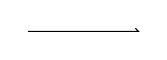
\begin{tikzpicture}\draw (0,0)--(1.4,0)--(1.36,.04);\end{tikzpicture}}

On va axiomatiser la situation de \deleted{\unsure{$A,A,\mathcal O$|$A,A_1,\mathcal O$}} $\mathrm{Tr}_{A_1\otimes A_2/A}$ et $N_{A_1\otimes A_2/A}$, en \unsure{considérant|explicitant|aboutit à|oubliant} la situation d'un anneau de base $k$, \inserted{et} d'une $k$-algèbre $A$ qui ``se comporte comme si c'\unsure{étais|était} une algèbre quadratique sur $k$'' (i.e. loc. libre de \unsure{rg|rang} $2$). Mais on ne suppose ni que $A$ soit loc. libre \deleted{\unsure{sur}} \inserted{ni $=$ plat} $/k$, ni que

\[
\alpha:k\longrightarrow A\qquad\lambda\longmapsto\lambda.1_A
\]

soit injective. Au lieu de cela, on suppose données \unsure{des|deux} applications

\[
\begin{aligned}
t_{A/k}=t &: A\longrightarrow k &\text{trace relative.}\\
n_{A/k}=n &: A\longrightarrow k &\text{norme relative,}
\end{aligned}
\]

satisfaisant les conditions suivantes

\textcircled{a} $t$ est linéaire, $n$ est quadratique, et $t$ se déduit de $n$ comme

\[
t(x)=\varphi_n(x,1)\qquad\text{$\varphi_n$ forme bil. ass. à $n$}
\]

donc on a \deleted{\unsure{équiv.}}

\[
\boxed{n(x+\unsure{\lambda_A|\lambda.1_A|\lambda1_A})=n(x)+\lambda^2\underset{\substack{\Vert\\1\ \text{cf. ci-dessous b)}}}{n(1)}+\lambda t(x)}
\]

% archive sheet number: 106

\scanpage{108}

\deleted{Il \unsure{s'ensuit} que, la forme} \inserted{\uline{NB} On \unsure{verra} plus bas comment la forme bil. $\varphi_n$} s'explicite \uline{en} termes de \deleted{\unsure{t|la}} la forme tr.

\[
\text{\textcircled{b}}\quad\boxed{\boxed{n(1)=1,\qquad n(xy)=n(x)n(y)}}
\]

\margin{i.e. $n$ est \deleted{\unsure{un}} hom de monoïdes unitaires $A^*\longrightarrow k^*$}

\textcircled{\deleted{b}c} \deleted{\unsure{T.q.}\ \unsure{Posons}} \inserted{D'où via a), y faisant $x=1$}

\[
\boxed{t(1)=2}
\]

Posons $\tau(f)=\alpha(t(f))$, et considérons l'application

\[
\sigma:f\longmapsto\bar f=\tau(f)-f
\]

\deleted{On voit que cette application, qui est} On a

\[
\tau(\bar f)=\tau(f)\underbrace{\tau(1)}_{2}-\tau(f)=\tau(f)
\]

\[
\begin{aligned}
\text{d'où}\qquad(\bar f)^{-}&=\tau(\bar f)-\bar f=f\\
\text{i.e.}\qquad\deleted{\sigma\ \mathrm{est}}\quad\sigma^2&=\mathrm{id}_A.
\end{aligned}
\]

\margin{Notons que par définition $\boxed{\deleted{\unsure{t(f)}}\tau(f)\overset{\mathrm{def}}{=}\alpha(t(f))=f+\bar f}$ et on a $\bar1=1$}

Ceci posé, on veut que l'on ait

1°) $\sigma$ \uline{est un} autom. d'algèbre, i.e.

\[
\boxed{\boxed{\sigma(xy)=\sigma(x)\sigma(y)}}\qquad x,y\in A
\]

ce qui s'explicite aussi

\[
2xy=\underset{\substack{\Vert\\\varphi_n(x,\bar y)\longrightarrow\text{voir d) ci-dessous}}}{\tau(xy)}
\inserted{-\tau(x)\tau(y)}+x\tau(y)+y\tau(x)
\]

\margin{comb. lin. (à coeff. dans $k$) de $1,x,y$}

\uline{NB} Au facteur $2$ près (qui n'est gênant qu'\deleted{\unsure{en car.|en car. 2}} si $2$ n'est pas inv. ds $k$), on voit donc que la structure d'algèbre de $A$ est connue quand on connaît $A$ en \deleted{\unsure{tant}} que $k$-module, avec l'élément $1_A$ et \unsure{d'où} \deleted{\unsure{on}} $\alpha:k\longrightarrow A$ par $\lambda\longmapsto\lambda.1_A$) et des \deleted{\unsure{linéaires}}\inserted{appl.} $t:A\longrightarrow k$, $n:A\longrightarrow k$.

% slanted
\margin{\uline{NB} Quand $\alpha$ est injectif, alors la formule \unsure{ci-contre} $\alpha(n(x))=x\bar x$ implique \unsure{alors} les formules de \textcircled{b} ci-dessus $n(xy)=n(x)n(y)$, $n(1)=1$}

\[
\text{2°)}\quad\boxed{\boxed{\alpha(\deleted{\unsure{N}}n(x))=x\bar x}}
\]

qui implique $\alpha(n(x))=\alpha(\overline{n(x)})$, mais en \deleted{\unsure{a donc}} fait

\[
\deleted{\unsure{2)}}\quad\boxed{n(\bar x)=n(\overset{\unsure{\leftarrow|-}}{x})}
\]

Car

\[
n(\bar x)=n(\deleted{\unsure{x}}\lambda.1-x)\underset{\substack{\text{où }\lambda=t(x)\\\mathrm{cf}\ \text{\textcircled{a}}}}{=}
n(x)+\deleted{\unsure{t(x)}}\lambda^2-\lambda t(x)\qquad\text{où }\lambda=t(x)
\]

donc on a bien $n(\bar x)=n(x)$

% archive sheet number: 107

\scanpage{109}

La formule ci-dessus pour

\[
\deleted{\unsure{\text{élémt}}}\quad\alpha(n(x)=\unsure{o|x}\bar x
\]

donne, si on fait $x=y+z$

\[
\begin{aligned}
\alpha(\underset{\substack{\Vert\\ n(y)+n(z)+\varphi_n(y,z)}}{\underbrace{n(y+z)}})
&=\deleted{\unsure{\alpha(n(x))}}(y+z)\overline{(y+z)}=\\
&=\underset{\substack{\Vert\\\alpha(n(y))}}{y\bar y}
+\underset{\alpha(n(z))}{z\bar z}
+\underbrace{y\bar z+\underbrace{z\bar y}_{=\overline{y\bar z}}}_{\tau(y\bar z)}
\end{aligned}
\]

\[
\text{\unsure{d'où|donc}}\qquad\alpha(\varphi_n(y,z))=\deleted{\unsure{\alpha t}}\tau(y\bar z)
\qquad\text{i.e.}\quad\alpha(t(y\bar z))
\]

donc si $\alpha$ est injectif, on en déduit

\[
\boxed{\varphi_n(y,z)=t(y\bar z)}
\]

i.e. la formule d'additivité pour $n$

\[
\boxed{n(y+z)=n(y)+n(z)+\underset{\substack{\Vert\\t(\bar yz)}}{t(y\bar z)}}
\qquad\text{car }t(x)=t(\bar x)
\]

Ceci posé, on veut

3°) la formule précédente est vraie (sans supposer $\alpha$ injective \ldots)

4°) Une formule facultative, quand $k$ est fini loc. libre \deleted{de} rang \deleted{\unsure{2}} $n$ sur un anneau $k_0$, et \deleted{alors on \unsure{ne} suppose} $A$ loc. libre de rang $2n$ sur $k_0$ (N.B. Donc $k_0\longrightarrow A$ injectif, mais on ne suppose pas $k\longrightarrow A$ injectif).

\[
\boxed{\left\{\begin{aligned}
\mathrm{Tr}_{k/k_0}(t(x))&=\mathrm{Tr}_{A/k_0}(x)\\
N_{k/k_0}(\deleted{\unsure{t}}n(x)&=N_{A/k_0}(x)
\end{aligned}\right.}
\]

\margin{identité entre applic. \uline{linéaires} $A\longrightarrow k_0$}

\margin{identité \unsure{de|des} $(2n)$-formes}

% archive sheet number: 108

\scanpage{110}

Récapitulons le formulaire pour

\diagram{\begin{tikzcd}[ampersand replacement=\&,column sep=large]
k\arrow[r,"{\deleted{\unsure{a}}\alpha}"] \& A\ (\text{$k$-alg})\arrow[l,bend left=17,"t"]\arrow[l,bend left=42,"n"]
\end{tikzcd}}

\margin{$\alpha$ hom d'anneaux comm. $\alpha(\lambda)=\lambda.1_A$ On pose $\tau(x)=\alpha t(x)$ \ $\nu(x)=\alpha n(x)$}

\textcircled{1} $t$ \deleted{\unsure{est|$k$}} $k$-linéaire, $\boxed{t(1_A)=2}$

\textcircled{2} $\deleted{\unsure{\xi}}x\longmapsto\bar x\overset{\mathrm{def}}{=}\tau(x)-x:A\longrightarrow A$ est un automorphisme d'alg., i.e. on a

\margin{(autom. involutif du $k$-module $A$, avec $\bar1_A=1_A$)}

\[
\boxed{\overline{xy}=\bar x\bar y}\qquad\text{i.e.}\quad
2xy=(\tau(xy)-\tau(x)\tau(y))+\tau(y)x+\tau(x)y
\]

\[
\text{\textcircled{3}}\quad\boxed{\left\{\begin{aligned}
n(\lambda x)&=\lambda^2n(x)\\
n(x+y)&=n(x)+n(y)+t(x\bar y)
\end{aligned}\right.}\qquad\lambda\in k,\ x\in A
\]

i.e. $n$ est quadratique, la forme bil. ass. est ici

\[
\varphi_n(x,y)=t(\unsure{x\bar y|y\bar x})
\]

\textcircled{4} $\boxed{n(1)=1}$ (\uline{NB} compte \deleted{\unsure{tenu}} de la formule d'additivité du 3°, cela implique $t(1)=2$)

\textcircled{5} $\boxed{\alpha(n(x))=x\bar x}$ $(x\in A)$ qui implique 3°, 4° si $\alpha$ injectif

\textcircled{6} (\uline{facultatif}, \deleted{)}\inserted{et} si $k$ loc. libre de rang $n$ sur $k_0$, et $A$ loc. libre de rang $2n$ sur $k_0$)

\[
\boxed{\begin{aligned}
\mathrm{Tr}_{k/k_0}(t(x))&=\mathrm{Tr}_{A/k_0}(x)\\
N_{k/k_0}(n(x))&=N_{A/k_0}(x)
\end{aligned}}\qquad x\in A
\]

La donnée de \inserted{\unsure{$\uparrow$} $A$ sur $k$ avec} $\alpha,t,n$ satisfaisant 1° à 5° sera appelée algèbre \uline{quasi-quadratique} sur $k$.

On va maintenant pouvoir étudier la situation \inserted{quasi-}\uline{biquadratique}

% archive sheet number: 109

\scanpage{111}

Données

a) anneau de base $k$

b) $k$-algèbres $A_1,A_2,A_3,A$

c) Sur chacune des $A_i$, structure quasi-quadratique sur $k$, i.e. on a

\diagram{\begin{tikzcd}[ampersand replacement=\&]
A_i\arrow[r,shift left,"t_i"]\arrow[r,shift right,"n_i"'] \& k
\end{tikzcd}}

\deleted{\unsure{(on pose :|Comme pour}}

satisfaisant les conditions 1° à 5° ci-dessus. On notera \deleted{\unsure{$\sigma_i$}} $x\longrightarrow\bar x$ l'involution canonique de $A_i$,

\[
\bar x=t_i(x)-x
\]

(NB on identifie \inserted{\deleted{$\bar x=t_i$} par abus de \unsure{notation|notations}} $\lambda\in k$ avec ses images ds les $A_i$, sans forcément supposer $k\longrightarrow A_i$ injectif\ldots)

d) Des Hom de $k$-algèbres

\diagram{\begin{tikzcd}[ampersand replacement=\&]
A_1\arrow[dr,"\alpha_1"] \& A_2\arrow[d,"\alpha_2"] \& A_3\arrow[dl,"\alpha_3"']\\
\& A \&
\end{tikzcd}}

(pas néc. inj.), et des structures d'alg. quasi-quadratiques de $A$ sur les $A_i$

\diagram{\begin{tikzcd}[ampersand replacement=\&,column sep=small]
\& A\arrow[dl,shift right,"T_1"']\arrow[dl,shift left,"N_1"]\arrow[d,shift right,"T_2"']\arrow[d,shift left,"N_2"]\arrow[dr,shift right,"T_3"']\arrow[dr,shift left,"N_3"]\&\\
A_1\&A_2\&A_3
\end{tikzcd}}

\diagram{\begin{tikzcd}[ampersand replacement=\&]
\&\deleted{A}\arrow[dl,shift right,"{\deleted{T_1}}"']\arrow[dl,shift left,"{\deleted{\unsure{N_1|\alpha_1}}}"]\arrow[d,shift right,"{\deleted{T_{\unsure{2}}}}"']\arrow[d,shift left,"{\deleted{N_2}}"]\\
\deleted{A_1}\&\deleted{\unsure{A_3|A_2}}
\end{tikzcd}}

chacune satisfaisant \deleted{\unsure{aux|donc}} au formulaire ci-dessus de 1° à 5°. De plus, \uline{compatibilité des trois}.

\deleted{On pose $\sigma_i(x)=T_i(x)-x$ et on veut que}

\margin{\deleted{$\sigma_i$ est un autom. involutif de $A$\unsure{?!|?|!|.|;}}}

\[
\deleted{\boxed{\sigma_1\sigma_2=\sigma_3,\ \sigma_2\sigma_3=\sigma_{\unsure{1|7}},\ \sigma_3\sigma_1=\sigma_2}}
\]

\deleted{i.e. que les $\sigma_i$ sont des involutions qui \uline{commutent} entre elles, et $\boxed{\sigma_1\sigma_2\sigma_3=\mathrm{id}}$}

% archive sheet number: 110

\scanpage{112}

Considérons un des 6 diagrammes comm.

\diagram{\begin{tikzcd}[ampersand replacement=\&]
 A_1 \arrow[r,dash,"\alpha_1"] \arrow[d,dash] \& A \arrow[d,dash,"\alpha_2"]\\
 k \arrow[r,dash] \& A_2
\end{tikzcd}}

on veut que la situation soit, du pt de vue \unsure{norme et|naïvement} trace, comme si $A_1$ était \unsure{une alg.} quadratique de $k$, et que $A$ en soit déduit \unsure{par} le changemt de base $k\longrightarrow A_2$.

% slanted
\margin{Mais on ne suppose ni $A_1/k$ ni $A/A_2$ \unsure{soit|sont|$(\alpha_2)$} \unsure{alg.|quasi-} quadratique, ni que $A_1,A_2$ \unsure{engendrent} la \unsure{$k$-alg. $A$}}

\[
 \boxed{T_2\bigl(\alpha_1(x_1)\deleted{\unsure{\alpha_1|\alpha_2}(x_2)}\bigr)=t_1(x_1)\deleted{\alpha_2(x_2)}} \tag*{\textcircled{$1^\circ$}}
\]

\margin{ce qui détermine $T_2$ sur $k[A_1,A_2]\subset A$ en termes de $t_1$}

i.e. on \unsure{veut|exige}\deleted{\unsure{p|pp}} un diagramme comm.

\diagram{\begin{tikzcd}[ampersand replacement=\&,column sep=large]
 A_1\otimes_k A_2 \arrow[r] \arrow[d,"t_1\otimes\mathrm{id}_{A_2}"'] \& A \arrow[d,"T_1"]\\
 A_2 \arrow[r,equal] \& A_2
\end{tikzcd}}

\margin{NB. $A_1\otimes A_2\longrightarrow A$ n'est \unsure{bien|pas} supposé injectif, mais que $t_1\otimes\mathrm{id}_{A_2}$ s'annule \unsure{au} moins \deleted{\unsure{sur}} \unsure{en|son|le} noyau}

Ceci implique que

\[
 \boxed{\sigma_2(\unsure{\alpha_1(x)|\alpha_1(x_1)})=\alpha_1(\bar x)}
\]

i.e $\sigma_2$ (\deleted{\unsure{et}} \unsure{et non|ou non|ainsi que} $\sigma_3$) ``induit'' sur $A_1$ l'involution donnée $x_1\longrightarrow\bar x_1$ de $A_1$

On veut une condition similaire pour les normes

\[
 \boxed{\boxed{N_2\bigl(\alpha_1(x_1)\deleted{\unsure{\alpha_2(x_2)}}\bigr)=n_1(x_1)\deleted{\unsure{\alpha_2(x_2)^2}}}} \tag*{\textcircled{$2^\circ$}}
\]

% archive sheet number: 111

